
%(BEGIN_QUESTION)
% Copyright 2010, Tony R. Kuphaldt, released under the Creative Commons Attribution License (v 1.0)
% This means you may do almost anything with this work of mine, so long as you give me proper credit

Suppose a voltmeter registers 0 volts between test points {\bf C} and {\bf B} in this circuit:

$$\includegraphics[width=15.5cm]{i03156x01.eps}$$

Identify the likelihood of each specified fault for this circuit.  Consider each fault one at a time (i.e. no coincidental faults), determining whether or not each fault could independently account for {\it all} measurements and symptoms in this circuit.

% No blank lines allowed between lines of an \halign structure!
% I use comments (%) instead, so that TeX doesn't choke.

$$\vbox{\offinterlineskip
\halign{\strut
\vrule \quad\hfil # \ \hfil & 
\vrule \quad\hfil # \ \hfil & 
\vrule \quad\hfil # \ \hfil \vrule \cr
\noalign{\hrule}
%
% First row
{\bf Fault} & {\bf Possible} & {\bf Impossible} \cr
%
\noalign{\hrule}
%
% Another row
$R_1$ failed open &  &  \cr
%
\noalign{\hrule}
%
% Another row
$R_2$ failed open &  &  \cr
%
\noalign{\hrule}
%
% Another row
$R_3$ failed open &  &  \cr
%
\noalign{\hrule}
%
% Another row
$R_4$ failed open &  &  \cr
%
\noalign{\hrule}
%
% Another row
$R_1$ failed shorted &  &  \cr
%
\noalign{\hrule}
%
% Another row
$R_2$ failed shorted &  &  \cr
%
\noalign{\hrule}
%
% Another row
$R_3$ failed shorted &  &  \cr
%
\noalign{\hrule}
%
% Another row
$R_4$ failed shorted &  &  \cr
%
\noalign{\hrule}
%
% Another row
Current source dead &  &  \cr
%
\noalign{\hrule}
} % End of \halign 
}$$ % End of \vbox


\vfil 

This question is typical of those in the ``Fault Analysis of Simple Circuits'' worksheet found in the {\it Socratic Instrumentation} practice worksheet collection, except that all answers are provided for those questions.  Feel free to use this practice worksheet to supplement your studies on this very important topic.

\underbar{file i03156}
\eject
%(END_QUESTION)





%(BEGIN_ANSWER)

This is a graded question -- no answers or hints given!

%(END_ANSWER)





%(BEGIN_NOTES)

A zero-voltage measurement across a load device where there ought to be voltage dropped means only one of two possibilities: either that load has no current passing through it, or it has failed shorted.  Thus, we are looking out for any possible fault that would either block current from reaching $R_2$, bypass current around $R_2$, or a shorted fault in $R_2$ itself:

% No blank lines allowed between lines of an \halign structure!
% I use comments (%) instead, so that TeX doesn't choke.

$$\vbox{\offinterlineskip
\halign{\strut
\vrule \quad\hfil # \ \hfil & 
\vrule \quad\hfil # \ \hfil & 
\vrule \quad\hfil # \ \hfil \vrule \cr
\noalign{\hrule}
%
% First row
{\bf Fault} & {\bf Possible} & {\bf Impossible} \cr
%
\noalign{\hrule}
%
% Another row
$R_1$ failed open & $\surd$ &  \cr
%
\noalign{\hrule}
%
% Another row
$R_2$ failed open &  & $\surd$ \cr
%
\noalign{\hrule}
%
% Another row
$R_3$ failed open & $\surd$ &  \cr
%
\noalign{\hrule}
%
% Another row
$R_4$ failed open &  & $\surd$ \cr
%
\noalign{\hrule}
%
% Another row
$R_1$ failed shorted &  & $\surd$ \cr
%
\noalign{\hrule}
%
% Another row
$R_2$ failed shorted & $\surd$ &  \cr
%
\noalign{\hrule}
%
% Another row
$R_3$ failed shorted &  & $\surd$ \cr
%
\noalign{\hrule}
%
% Another row
$R_4$ failed shorted & $\surd$ &  \cr
%
\noalign{\hrule}
%
% Another row
Current source dead & $\surd$ &  \cr
%
\noalign{\hrule}
} % End of \halign 
}$$ % End of \vbox



%INDEX% Troubleshooting review: electric circuits

%(END_NOTES)


